%%%%%%%%%%%%%%%%%%%%%%%%%%%%%%%%%%%%%%%%%%%%%%%%%%%%%%%%%%%%%%%%%%%%
% Documento de diseño e investigación del Proyecto 4, EL-4201 Procesamiento Electrónico de Potencia
% Compilar con make. Los datos que todavía no existen van con \pendiente{...}
%%%%%%%%%%%%%%%%%%%%%%%%%%%%%%%%%%%%%%%%%%%%%%%%%%%%%%%%%%%%%%%%%%%%

\documentclass[journal]{IEEEtran}
% Preámbulo común del documento de diseño y del informe técnico de PEDP
\usepackage{instructivo}
\renewcommand{\IEEEkeywordsname}{Palabras clave}
\usepackage[american,siunitx]{circuitikz}

\sisetup{per-mode=symbol, group-digits=integer, output-decimal-marker={,}}
\graphicspath{{./}{./fig/}}

\usepackage{amsmath}
\usepackage{float}
\usepackage[natbib=true,style=trad-unsrt,backend=biber]{biblatex}
\addbibresource{literatura.bib}
\renewcommand*{\bibfont}{\footnotesize}

% Columnas de tabularx que parten el texto en varias líneas para no salirse de la columna
\newcolumntype{L}{>{\raggedright\arraybackslash}X}
\newcolumntype{C}{>{\centering\arraybackslash}X}

% Marcador visible para datos que todavía no existen, nunca se llena con un valor calculado
\newcommand{\pendiente}[1]{\textcolor{red}{\textbf{[#1]}}}

\hyphenation{op-tical net-works semi-conduc-tor}


\begin{document}
\deactivatequoting
\title{Diseño del control de corriente de un inversor monofásico en puente H con regulador PR discreto}

\author{Jefferson~Chinchilla~Q.,~\IEEEmembership{Estudiante,~ITCR,}
	Nicolás~Mena~V.,~\IEEEmembership{Estudiante,~ITCR,}
	y~Mattio~Coghi~Q.,~\IEEEmembership{Estudiante,~ITCR}
}

\markboth{Procesamiento Electrónico de Potencia, IIS2026}%
{Proyecto 4: control de corriente con regulador PR}

\maketitle

\begin{abstract}
	Se diseñó un inversor monofásico en puente H con modulación PWM unipolar a \SI{20}{kHz}, alimentado con \SI{18}{V}, que alimenta una carga $R$--$L$ de \SI{12}{\ohm} y \SI{30}{mH}, y se sintonizó un regulador proporcional-resonante discreto para que la corriente siga una referencia de \SI{50}{Hz} de \num{0.2}, \num{0.5} y \SI{1.0}{A} pico. El regulador cruza en \SI{1}{kHz} con \ang{66.5} de margen de fase y \SI{10.5}{dB} de margen de ganancia, y en simulación el error de amplitud de la fundamental queda entre \num{5.3} y \SI{2.9}{\percent} en los cinco períodos siguientes a un escalón. El escalón de amplitud aplicado lejos del cruce por cero satura el puente, y se resolvió con una rampa de un período en la referencia. El tiempo muerto de \SI{1}{\micro s} baja la corriente en lazo abierto entre \num{7} y \SI{27}{\percent}, según la referencia.
\end{abstract}


\begin{IEEEkeywords}
	Controlador proporcional-resonante, inversor en puente H, modulación unipolar, tiempo muerto.
\end{IEEEkeywords}

\section{Introducción}
\label{sec:intro}
\IEEEPARstart{L}{a} corriente que entrega un inversor a una carga inductiva se controla con un lazo cerrado, y cuando la referencia es senoidal un regulador PI deja error de amplitud y de fase, porque su ganancia solo es infinita en continua. El regulador proporcional-resonante (PR) pone la ganancia infinita en la frecuencia de la referencia y se ejecuta sin transformar a ejes sincrónicos, lo que lo hace barato de correr en un procesador sin hardware de control dedicado \cite{teodorescu2006}.

Este informe cubre el componente de potencia del Proyecto 4. Se describen el puente H y su cadena de compuertas, la carga y el sensor de corriente, el modelo de la planta, la sintonización y discretización del PR, y el plan de validación. El PR se ejecuta en un MicroBlaze V sobre una Basys~3, y esa parte digital se documenta en el informe del curso de Taller de Diseño Digital. Aquí solo se tratan las interfaces con ella, la señal PWM, el instante de muestreo y el período de control.

Los criterios que debe cumplir el sistema son un error relativo de amplitud de la fundamental menor a \SI{10}{\percent} en una ventana de al menos cinco períodos de \SI{50}{Hz} para referencias de \num{0.2}, \num{0.5} y \SI{1.0}{A} pico, y un rizado de conmutación menor a \SI{0.20}{A} pico a pico. Además se evalúan los cambios de referencia de \num{0.2} a \num{0.5} y de \num{0.5} a \SI{1.0}{A}, y un cambio de la resistencia de al menos \SI{25}{\percent} con \SI{0.5}{A}.

\section{Parámetros del sistema}
\label{sec:param}
La tensión de bus es $V_{dc}=\SI{18}{V}$, punto medio del rango de \num{12} a \SI{24}{V} que permite el enunciado. Se eligió así porque con \SI{12}{V} el índice de modulación que pide \SI{1.0}{A} queda demasiado cerca del límite de saturación, y con \SI{24}{V} el rizado y las pérdidas suben sin necesidad. Las protecciones se dimensionan con \SI{24}{V}, para que un ajuste equivocado de la fuente no las deje cortas.

La frecuencia de conmutación es $f_{sw}=\SI{20}{kHz}$, y el lazo muestrea una vez por período de portadora, $T_s=\SI{50}{\micro s}$. La carga vigente es $R=\SI{12}{\ohm}$ y $L=\SI{30}{mH}$, un transformador usado como inductor. Estos valores son nominales, los que se dictaron para armar el banco, y la medición de $L$ y $R$ totales está \pendiente{medir $L$ y $R$ totales}. Con ellos, a \SI{50}{Hz}, $|Z|=\SI{15.26}{\ohm}$ y la corriente atrasa \ang{38.1} respecto de la tensión.

El tiempo muerto es $T_M=\SI{1}{\micro s}$ y la precarga del bootstrap dura \SI{70}{\micro s}. Los demás parámetros, junto con su justificación, están en las secciones que siguen.

\section{Etapa de potencia}
\label{sec:potencia}

\subsection{Puente H y modulación}
\label{sec:puente}
El puente tiene dos piernas, cada una con un MOSFET alto y uno bajo (Fig.~\ref{fig:puente}). La carga ve $v_o=v_A-v_B$, con valores $+V_{dc}$, \num{0} y $-V_{dc}$. En la modulación unipolar las dos piernas se comparan contra la misma portadora triangular, la A contra $d$ y la B contra $-d$, de modo que el promedio sobre un período de conmutación es $\bar v_o=V_{dc}\,d$ mientras $|d|\le1$ \cite{mohan2003power}. Cada transistor conmuta a $f_{sw}$, pero la tensión sobre la carga pulsa a $2f_{sw}$, porque en cada semiciclo hay dos pulsos por período. Con el índice de modulación $m_a=V_{m,ref}/V_{m,portadora}\le1$, la fundamental de la tensión es $V_1\approx m_aV_{dc}$, y el primer armónico importante queda en $2f_{sw}$ (Fig.~\ref{fig:unipolar}).

\begin{figure}[!ht]
	\centering
	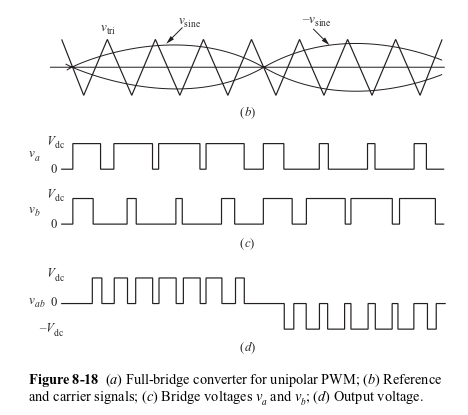
\includegraphics[width=0.9\columnwidth]{unipolar_pwm}
	\caption{Funcionamiento del PWM unipolar.}
	\label{fig:unipolar}
\end{figure}

\begin{figure}[!ht]
	\centering
	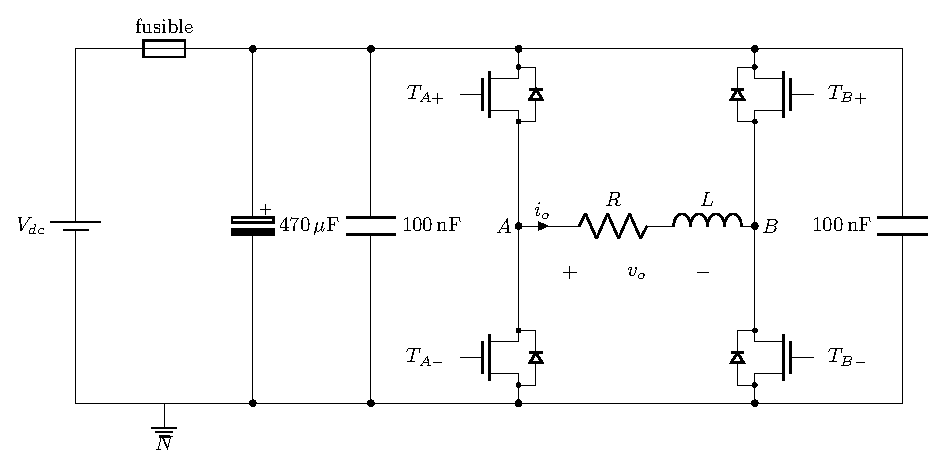
\includegraphics[width=\columnwidth]{puente_h}
	\caption{Puente H con la carga $R$--$L$, el fusible y los capacitores del bus.}
	\label{fig:puente}
\end{figure}

\subsection{MOSFET y pérdidas}
\label{sec:mosfet}
Los cuatro interruptores son IRF520N de canal N, de \SI{100}{V} y \SI{9.7}{A} continuos \cite{irf520n}. Con $V_{dc}$ hasta \SI{24}{V} se pide $V_{DS}\ge\SI{40}{V}$, que cubre el sobrepico $L\,di/dt$ de la inductancia parásita del bus y la energía que la carga devuelve en parte de cada período. Con el regulador saturado en \num{0.92}, la corriente de falla queda acotada en $0.92\,V_{dc}/R=\SI{1.84}{A}$ con \SI{24}{V}, más de tres veces por debajo de los \SI{6.8}{A} que el dispositivo soporta a \SI{100}{\celsius}.

Con \SI{24}{V} y \SI{1}{A} pico, cada transistor disipa unos \SI{0.31}{W} a \SI{20}{kHz} y \SI{0.52}{W} a \SI{40}{kHz}. El término mayor es la recuperación inversa del diodo de cuerpo, $Q_{rr}V_{dc}f_{sw}$, y la conducción ($I_{rms}^2R_{DS(on)}$, \SI{0.1}{W}) y la conmutación ($\tfrac12V_{dc}I(t_r+t_f)f_{sw}$, \SI{24}{mW} a \SI{20}{kHz}) pesan menos. Con $R_{\theta JA}=\SI{62}{\celsius/W}$ la unión sube unos \SI{32}{\celsius} sobre el ambiente sin disipador. Las tres cifras son cotas, porque los datos de la hoja están medidos con corrientes mayores a las de este montaje.

\subsection{Drivers, aislamiento y bootstrap}
\label{sec:drivers}
Cada pierna usa un IR2110, con las cuatro entradas referidas a la tierra de potencia, y el lado flotante de la compuerta alta se alimenta con un bootstrap \cite{ir2110}. Cada salida llega a su MOSFET por \SI{10}{\ohm}, que limita el pico de compuerta a \SI{1.5}{A} contra los \SI{2}{A} mínimos que garantiza el driver. El capacitor de bootstrap es de \SI{470}{nF}, unas tres veces el mínimo de \SI{156}{nF} que sale de la carga de compuerta y las corrientes de reposo en el peor caso (\SI{10}{kHz}), y su diodo es un 1N4148 con \SI{22}{\ohm} en serie que limita la primera carga a \SI{0.65}{A} \cite{1n4148}.

La tierra de la Basys~3 y la del puente están separadas. Cada una de las cuatro compuertas cruza la barrera con un optoacoplador VO3120 \cite{vo3120}, activado por un PN2222A desde el pin del Pmod \cite{pn2222a}. La polaridad es tal que un pin en alta impedancia, un cable suelto o la placa sin alimentar dejan el LED apagado y la compuerta apagada. Una falla del lado de la FPGA no puede encender las cuatro compuertas y cortocircuitar las piernas. Los \SI{15}{V} del lado del puente salen de un canal aparte de la fuente, porque $V_{dc}$ varía de \num{12} a \SI{24}{V}.

La compuerta alta solo se repone mientras conduce la baja de la misma pierna. Con \SI{20}{kHz} y $T_M=\SI{1}{\micro s}$, el capacitor deja de recargarse cuando $d$ llega a $1-(T_M f_{clk}+100)/\mathrm{MAX}=\num{0.92}$, y por eso el regulador recorta su salida en $0.92$. El cálculo exige que la baja conduzca al menos \SI{1}{\micro s} por período.

Al pasar a operación, cada pierna enciende primero su compuerta baja durante \SI{70}{\micro s}, para que el capacitor llegue al \SI{99.4}{\percent} de su carga final en el peor caso de tolerancias (\SI{22}{\ohm} más \SI{5}{\percent}, \SI{470}{nF} más \SI{20}{\percent}, $5\tau\approx\SI{68}{\micro s}$). Mientras tanto la carga ve \SI{0}{V}, y no hay camino entre $V_{dc}$ y tierra.

\subsection{Tiempo muerto}
\label{sec:tm}
Para que los dos transistores de una pierna no conduzcan a la vez se exige $T_M>t_{off}-t_{on}$ en el peor caso. El retardo común a los dos flancos se cancela en la resta, y lo que cuenta es la diferencia entre dos cadenas distintas. Sumando el peor caso de cada eslabón se obtiene \SI{813}{ns}.

\begin{itemize}
	\item PN2222A, \SI{250}{ns} de apagado.
	\item VO3120, \SI{0.3}{\micro s} de diferencia entre dos unidades, porque $t_{PHL}$ y $t_{PLH}$ van de \num{0.1} a \SI{0.4}{\micro s}.
	\item IR2110, \SI{125}{ns} de apagado.
	\item IRF520N, unos \SI{138}{ns}, estimados con la resistencia de compuerta total de \SI{17.5}{\ohm} y su capacidad de entrada.
\end{itemize}

Se fijó $T_M=\SI{1}{\micro s}$, que deja \SI{187}{ns} (\SI{23}{\percent}) para un tiempo de almacenamiento del transistor mayor al de la hoja y para el cableado. El flanco más lento de la cadena, el apagado, tarda unos \SI{0.91}{\micro s} entre el pin y el corte del MOSFET, dentro de los \SI{2}{\micro s} que se tomaron como retardo máximo de esa cadena para el lazo. Verificar los \SI{1}{\micro s} en el osciloscopio, con la potencia apagada, es una condición antes de energizar (Sección~\ref{sec:plan}).

\subsection{Protecciones}
\label{sec:prot}
Cada falla tiene su escala de tiempo, y la cubre la protección que alcanza a actuar. La conducción simultánea en una pierna dura nanosegundos y la evitan el tiempo muerto y la polaridad de la cadena. La sobrecorriente con la carga conectada dura cientos de microsegundos y la corta el software. Una falla sostenida la corta el límite de la fuente y el fusible.

\begin{itemize}
	\item Un electrolítico de \SI{470}{\micro F} y \SI{63}{V} en el bus y un capacitor de película de \SI{100}{nF} por pierna, junto a los transistores, que entrega la corriente de los flancos.
	\item Un fusible rápido de \SI{630}{mA} a la entrada. La fuente entrega unos \SI{0.39}{A} en promedio con \SI{1}{A} pico, y el fusible queda al \SI{62}{\percent} de su nominal.
	\item Límite de corriente de la fuente de \SI{0.52}{A} en los ensayos, y de \SI{0.1}{A} en la primera energización, que sube $V_{dc}$ desde cero.
	\item Límite de \SI{50}{mA} en el canal de \SI{15}{V}. Si entra en limitación, el VO3120 apaga las compuertas por subtensión.
\end{itemize}

El software baja las cuatro compuertas cuando la corriente medida supera \SI{1.3}{A}, y entre que la corriente cruza el umbral y las compuertas quedan en bajo pasan hasta dos períodos, \SI{100}{\micro s}. No existe un apagado por hardware a partir de una medición de corriente. Con la carga en cortocircuito no hay resistencia que acote la corriente, y el pico de la descarga del electrolítico llega a \SI{60}{A}, por encima de los \SI{38}{A} pulsados del IRF520N. Ese caso no queda cubierto para los MOSFET, y se mitiga solo limitando la fuente.

\section{Carga RL y sensor de corriente}
\label{sec:carga}

\subsection{Dimensionamiento de la carga}
\label{sec:dim}
La resistencia total fija la tensión que pide cada referencia. Con $|Z|=\SI{15.26}{\ohm}$ el índice pico $m=|Z|I/V_{dc}$ es \num{0.170}, \num{0.424} y \num{0.848} para \num{0.2}, \num{0.5} y \SI{1.0}{A}, todos bajo el tope de \num{0.92} del regulador. Con \SI{1.0}{A} el margen es de \SI{8}{\percent}, mucho más angosto que con una carga de \SI{10}{\ohm} y \SI{2}{mH}, donde el índice era \num{0.557}.

A \SI{1.0}{A} pico la potencia media en la resistencia total es $I_{rms}^2R=\SI{6}{W}$, que incluye el devanado y la resistencia externa. La parte que disipan las resistencias externas de \SI{5}{W} depende de cuánta resistencia sea del devanado, y está \pendiente{medir $R$ del devanado del transformador y repartir la potencia}.

El rizado máximo de conmutación es $\Delta i_{max}=V_{dc}/(8Lf_{sw})=\SI{3.75}{mA}$, quince veces menos que con la bobina de \SI{2}{mH}, así que con esta $L$ el rizado deja de restringir el diseño. A \SI{1.0}{A} el índice \num{0.848} está lejos de $d=0.5$, y el rizado real baja a \SI{1.9}{mA}.

\subsection{Criterios de diseño de la carga}
\label{sec:criterios}
Los criterios con que se dimensionó la carga los fijó Jefferson al armar el banco, con una bobina de \SI{2}{mH}, y se repiten aquí para evaluarlos contra la carga vigente. El índice de modulación pico que pide una referencia es $m_a=I\,|Z|/V_{dc}$. El regulador recorta en $m_{a,max}=0.92$ y se pidió un margen del \SI{20}{\percent} bajo ese tope, $m_a\le0.8\cdot0.92=0.736$, que con \SI{1.0}{A} y \SI{18}{V} da $|Z|\le\SI{13.2}{\ohm}$. Para el rizado, $L\ge V_{dc}/(8\,\Delta i_{max}f_{sw})=\SI{0.56}{mH}$ con \SI{0.20}{A} (Ec.~\ref{eq:rizado}).

Las resistencias externas son de \SI{5}{W} y se cargan hasta el \SI{50}{\percent}. Con $I_{rms}^2=\SI{0.5}{A^2}$ a \SI{1.0}{A} pico y $N$ resistencias en serie, $0.5\,R_{ext}/N\le\SI{2.5}{W}$, de donde $R_{ext}\le5N\,\si{\ohm}$, \SI{10}{\ohm} con dos y \SI{15}{\ohm} con tres. El tiempo muerto fija un piso para $R$. La pérdida de tensión de \SI{0.72}{V} tiene una fundamental de \SI{0.92}{V} (Sección~\ref{sec:tm_modelo}), y se pidió que no pase de la mitad de la tensión que exige la referencia menor, $R\ge0.92/(0.5\cdot0.2)=\SI{9.2}{\ohm}$, donde $R$ incluye el devanado, el shunt y los dos MOSFET. Por último, con el regulador saturado la corriente solo la limita la resistencia, $I_{max}=0.92\,V_{dc}/R$, y el inductor debe soportarla sin saturarse.

Evaluados con la carga vigente de \SI{12}{\ohm} y \SI{30}{mH}.

\begin{itemize}
	\item $|Z|\le\SI{13.2}{\ohm}$ no se cumple, porque $|Z|=\SI{15.26}{\ohm}$ y $m_a=0.848$ a \SI{1.0}{A}. El criterio se escribió sobre $R$ con una bobina de \SI{2}{mH}, donde $\omega L=\SI{0.63}{\ohm}$ no pesa, y con \SI{30}{mH} la reactancia de \SI{9.42}{\ohm} a \SI{50}{Hz} sí.
	\item $R\ge\SI{9.2}{\ohm}$ se cumple con \SI{12}{\ohm}.
	\item $L\ge\SI{0.56}{mH}$ se cumple por más de dos órdenes de magnitud.
	\item $I_{max}=\SI{1.38}{A}$ con \SI{18}{V}, y el umbral de falla de \SI{1.3}{A} queda debajo. La corriente de saturación del transformador está \pendiente{medir o buscar la corriente de saturación del transformador}.
	\item $R_{ext}\le5N\,\si{\ohm}$ depende de cuánta de la resistencia total es del devanado, \pendiente{medir $R$ del devanado}.
\end{itemize}

La carga original salió de estos criterios. Con $R=\SI{10}{\ohm}$ y $L=\SI{2}{mH}$, la resistencia externa son dos resistencias de \SI{4.7}{\ohm} y \SI{5}{W} en serie, $R_{ext}=\SI{9.4}{\ohm}$, y el resto es devanado, shunt y MOSFET. Con $|Z|=\SI{10.02}{\ohm}$ los tres puntos de operación quedaron como en la Tabla~\ref{tab:candidato}, todos bajo $m_a=0.736$ y bajo \SI{0.20}{A} de rizado, y cada resistencia de \SI{4.7}{\ohm} disipa \SI{2.35}{W}, el \SI{47}{\percent} de su nominal.

\begin{table}[!ht]
	\centering
	\caption{Puntos de operación de la carga original (\SI{10}{\ohm}, \SI{2}{mH}) con \SI{18}{V}. $P_{ext}$ es la potencia en las dos resistencias externas.}
	\label{tab:candidato}
	\begin{tabular}{ccccc}
		\toprule
		$I_{pico}$ (A) & $V_1$ (V) & $m_a$ & $\Delta i_{max}$ (A) & $P_{ext}$ (W) \\
		\midrule
		\num{0.2} & \num{2.00} & \num{0.111} & \num{0.022} & \num{0.19} \\
		\num{0.5} & \num{5.01} & \num{0.278} & \num{0.045} & \num{1.18} \\
		\num{1.0} & \num{10.02} & \num{0.557} & \num{0.056} & \num{4.70} \\
		\bottomrule
	\end{tabular}
\end{table}

El enunciado pide un cambio de al menos \SI{25}{\percent} en la resistencia externa con \SI{0.5}{A} pico. Con la carga original se agrega una resistencia de \SI{2.7}{\ohm} en serie, $R_{ext}=\SI{12.1}{\ohm}$, un cambio de $2.7/9.4=\SI{28.7}{\percent}$. Con la carga vigente y esa misma resistencia, $R$ pasa de \num{12} a \SI{14.7}{\ohm}, con $|Z|=\SI{17.46}{\ohm}$, $m_a=0.485$ y \SI{1.84}{W} en la resistencia total. Ambos puntos quedan dentro de los límites de tensión y de disipación, pero el cambio de la resistencia externa es del \SI{28.7}{\percent} solo si $R_{ext}$ sigue siendo \SI{9.4}{\ohm}, \pendiente{confirmar $R_{ext}$ vigente y el porcentaje del cambio}. Contra la resistencia total son \SI{22.5}{\percent}.

\subsection{Sensor y acondicionamiento}
\label{sec:sensor}
La corriente se mide con un ACS712 de \SI{5}{A} (\SI{185}{mV/A} típico, \num{180} a \SI{190}{mV/A}), un sensor de efecto Hall bidireccional con aislamiento propio \cite{acs712}, que a \SI{0}{A} entrega $V_{cc}/2=\SI{2.5}{V}$. El sensor necesita \SI{5}{V} y las salidas de la Basys~3 son de \SI{3.3}{V}, así que lleva una fuente aparte de \SI{5}{V}. El XADC de la Basys~3 solo acepta \SI{0}{} a \SI{1}{V} en el Pmod JXADC, así que un amplificador restador quita ese cero, aplica una ganancia $A_v$ y suma un offset de \SI{0.5}{V}, de modo que \SI{0}{A} cae a mitad de la escala útil. La salida del amplificador pasa por un filtro RC antialias.

\begin{figure}[!ht]
	\centering
	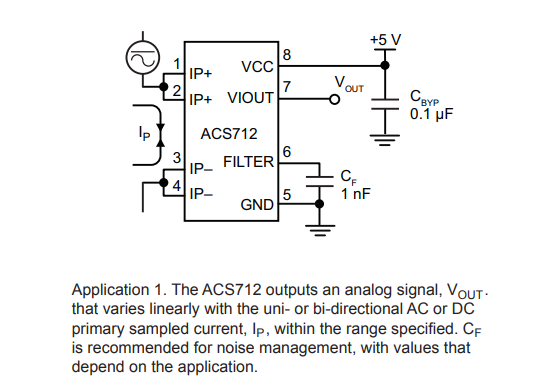
\includegraphics[width=\columnwidth]{circuito_medidor_de_corriente}
	\caption{Circuito de referencia del ACS712 para medir la corriente.}
	\label{fig:medidor}
\end{figure}

\begin{figure}[!ht]
	\centering
	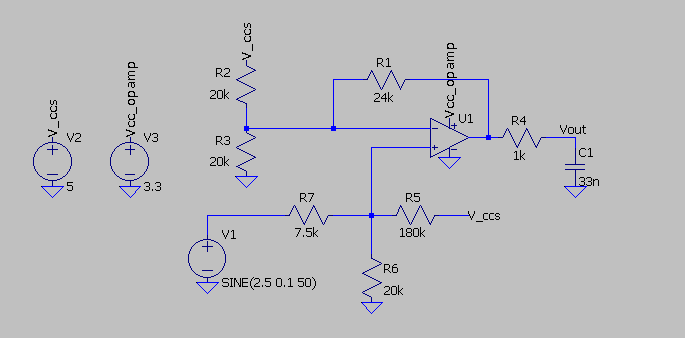
\includegraphics[width=\columnwidth]{circuito_acondicionador}
	\caption{Circuito acondicionador entre el sensor y el JXADC, con $R_1=\SI{24}{k\ohm}$ y $R_7=\SI{7.5}{k\ohm}$, la versión del diseño. El esquema de LTspice del 13 de noviembre tiene $R_1=\SI{12}{k\ohm}$ y $R_7=\SI{15}{k\ohm}$.}
	\label{fig:acond}
\end{figure}

El circuito tiene tres tareas, quitar el cero del sensor (\SI{2.5}{V}), amplificar la señal y poner un cero nuevo en \SI{0.5}{V} que deje representar corrientes negativas. Con $V_{off}=V_{cc}R_6/(R_5+R_6)$ y $R_+=R_5\parallel R_6$ en la entrada no inversora, y $V_m=V_{cc}R_3/(R_2+R_3)$ y $R_-=R_2\parallel R_3$ en la inversora, la ganancia es $A_v=(1+R_1/R_-)\,R_+/(R_++R_7)$. Si las dos ramas están balanceadas, $R_+/R_7=R_1/R_-=k$, la ganancia se reduce a $A_v=k$ y
\begin{equation}
	V_o=A_v\,(V_{sensor}-V_m)+V_{off}.
	\label{eq:acond}
\end{equation}

La ganancia se eligió para dejar \SI{0.10}{V} de margen en cada extremo del rango de \SI{0}{} a \SI{1}{V}, una excursión de $\pm\SI{0.40}{V}$ alrededor de \SI{0.5}{V}. Con la sensibilidad de \SI{100}{mV/A} del sensor y la corriente máxima de la carga original, \SI{1.66}{A}, $A_v\le0.40/(0.100\cdot1.66)=2.41$, y se tomó $A_v=2.4$. Con la carga vigente y el umbral de falla de \SI{1.3}{A} la cota es $A_v\le3.08$, y la ganancia de \num{2.4} la cumple igual. El offset de \SI{0.5}{V} sale de $R_5=9R_6$, con $R_6=\SI{20}{k\ohm}$ y $R_5=\SI{180}{k\ohm}$, que dan $R_+=\SI{18}{k\ohm}$. El balance pide $R_7=R_+/A_v=\SI{7.5}{k\ohm}$, y con $R_2=R_3=\SI{20}{k\ohm}$ y $R_1=\SI{24}{k\ohm}$ el amplificador queda balanceado. Con $V_{sensor}=\SI{2.5}{V}$ resulta $V_+=\SI{1.912}{V}$ y $V_o=\SI{0.50}{V}$.

Jefferson cambió $R_1$ a \SI{12}{k\ohm} y $R_7$ a \SI{15}{k\ohm} en el esquema del 13 de noviembre. El balance se mantiene ($R_+/R_7=R_1/R_-=1.2$) y con $V_{sensor}=\SI{2.5}{V}$ la salida sigue en \SI{0.50}{V}, pero la ganancia pasa a \num{1.2} y la sensibilidad de todo el camino a \SI{0.12}{V/A}. El texto de diseño no recoge ese cambio. En el banco se confirmó el 17 de noviembre que quedó montada la ganancia de \num{1.2}, y que el sensor instalado es el de \SI{5}{A}, no el de \SI{20}{A} con que se calculó $A_v=2.4$. La sensibilidad del sensor medida fue de \SI{183}{mV/A}, dentro de los \num{180} a \SI{190}{mV/A} de la hoja de datos \cite{acs712}, y la de todo el camino queda en $1.2\cdot\SI{183}{mV/A}=\SI{0.2196}{V/A}$.

Con la carga vigente el techo en régimen senoidal es $0.92\,V_{dc}/|Z|=\SI{1.085}{A}$ pico, y la escala del XADC sigue cubriendo el umbral de falla de \SI{1.3}{A} con cualquiera de las dos ganancias. Con \SI{0.2196}{V/A} el software usa $\SI{1}{V}/(4096\cdot\SI{0.2196}{V/A})=\SI{1.1118e-3}{A}$ por cuenta del XADC de \num{12} bits, y la escala cubre $\pm\SI{2.28}{A}$. Antes usaba provisionalmente \SI{0.3}{V/A} (\SI{8.138e-4}{A} por cuenta), que hacía leer al lazo el \SI{73}{\percent} de la corriente real. Cuando se mida la ganancia real se actualizan la conversión de cuentas a amperes y los límites de la protección. La calibración contra una sonda de corriente está \pendiente{calibrar el sensor contra la sonda}.

Para el offset se adopta la cuenta de \num{2048}, que es \SI{0.5}{V} en el XADC de \num{12} bits y \SI{1}{V} de escala. Sale del diseño del acondicionador de Jefferson, donde el restador quita los \SI{2.5}{V} del sensor y suma \SI{0.5}{V}, y es el valor que ya usa el software como \texttt{ADC\_OFFSET\_CUENTAS}. La hoja de datos del ACS712 \cite{acs712} da la salida a \SI{0}{A} solo como $V_{CC}\times0.5$ típico, sin mínimo ni máximo, y como deriva con la temperatura \SI{-0.08}{mV/\celsius} entre \SI{25}{} y \SI{150}{\celsius} para la versión de \SI{5}{A}, de modo que ni el offset de fábrica ni su dispersión están acotados por el fabricante. Con el banco a unos \SI{25}{\celsius} la deriva es de unos \SI{4}{mV} si el sensor sube \SI{60}{\celsius}, apenas \num{0.04}~A. Como el cero también sigue a $V_{cc}$, un error de \SI{50}{mV} en la fuente de \SI{5}{V} lo mueve \SI{25}{mV}, y ese corrimiento sí es comparable con la referencia de \SI{0.2}{A}. Con esa incertidumbre y sin cota del fabricante se adopta \num{2048} cuentas como el cero del sensor, y la protección y la conversión a amperes parten de ese valor.

El filtro antialias RC propuesto usa \SI{1}{k\ohm} y \SI{33}{nF}, con corte en \SI{4823}{Hz}, un retardo de \SI{33}{\micro s} y un atraso de $\arctan(50/4823)=\ang{0.59}$ sobre la señal de \SI{50}{Hz}. Se pidió un corte entre \num{2} y \SI{5}{kHz}, el rango aceptado para el regulador, porque un corte menor atenúa más ruido pero agrega más retardo al lazo. El ruido del sensor es de \SI{11}{mV} pico a pico con \SI{2}{kHz} de ancho de banda, y crece con la raíz del ancho de banda, así que con ese corte el ruido equivale a unos \SI{17}{mV}, \SI{0.17}{A} pico a pico con la sensibilidad de \SI{100}{mV/A}. La Tabla~\ref{tab:antialias} compara tres capacitores con $R_4=\SI{1}{k\ohm}$. El valor final se define con el ruido medido, \pendiente{medir ruido del sensor y fijar $C_1$}.

\begin{table}[!ht]
	\centering
	\caption{Opciones del filtro antialias con $R_4=\SI{1}{k\ohm}$.}
	\label{tab:antialias}
	\begin{tabular}{ccccc}
		\toprule
		$C_1$ (nF) & $f_c$ (Hz) & $t_d$ ($\mu$s) & Fase a \SI{50}{Hz} (°) & Ruido (A p-p) \\
		\midrule
		\num{80} & \num{1989} & \num{80} & \num{1.44} & \num{0.11} \\
		\num{53} & \num{3003} & \num{53} & \num{0.95} & \num{0.13} \\
		\num{33} & \num{4823} & \num{33} & \num{0.59} & \num{0.17} \\
		\bottomrule
	\end{tabular}
\end{table}

La Sección~\ref{sec:estab} muestra qué tanto margen cuesta cada corte. La columna de fase de la tabla del documento de diseño de Jefferson daba \num{0.195}, \num{0.288} y \ang{0.434}, que no coinciden con su propio $\arctan(50/f_c)$, y aquí se recalculó en Octave.

\subsection{Simulación del acondicionador}
\label{sec:sim_acond}
El acondicionador se simuló en LTspice con una entrada de \SI{2.5}{V} más una senoidal de \SI{0.1}{V} pico a \SI{50}{Hz}, que corresponde a \SI{1.0}{A} pico. La salida queda dentro de \SI{0}{} a \SI{1}{V}, con el cero en \SI{0.5}{V}, que es lo que recibe el XADC (Fig.~\ref{fig:acond_sim}).

\begin{figure}[!ht]
	\centering
	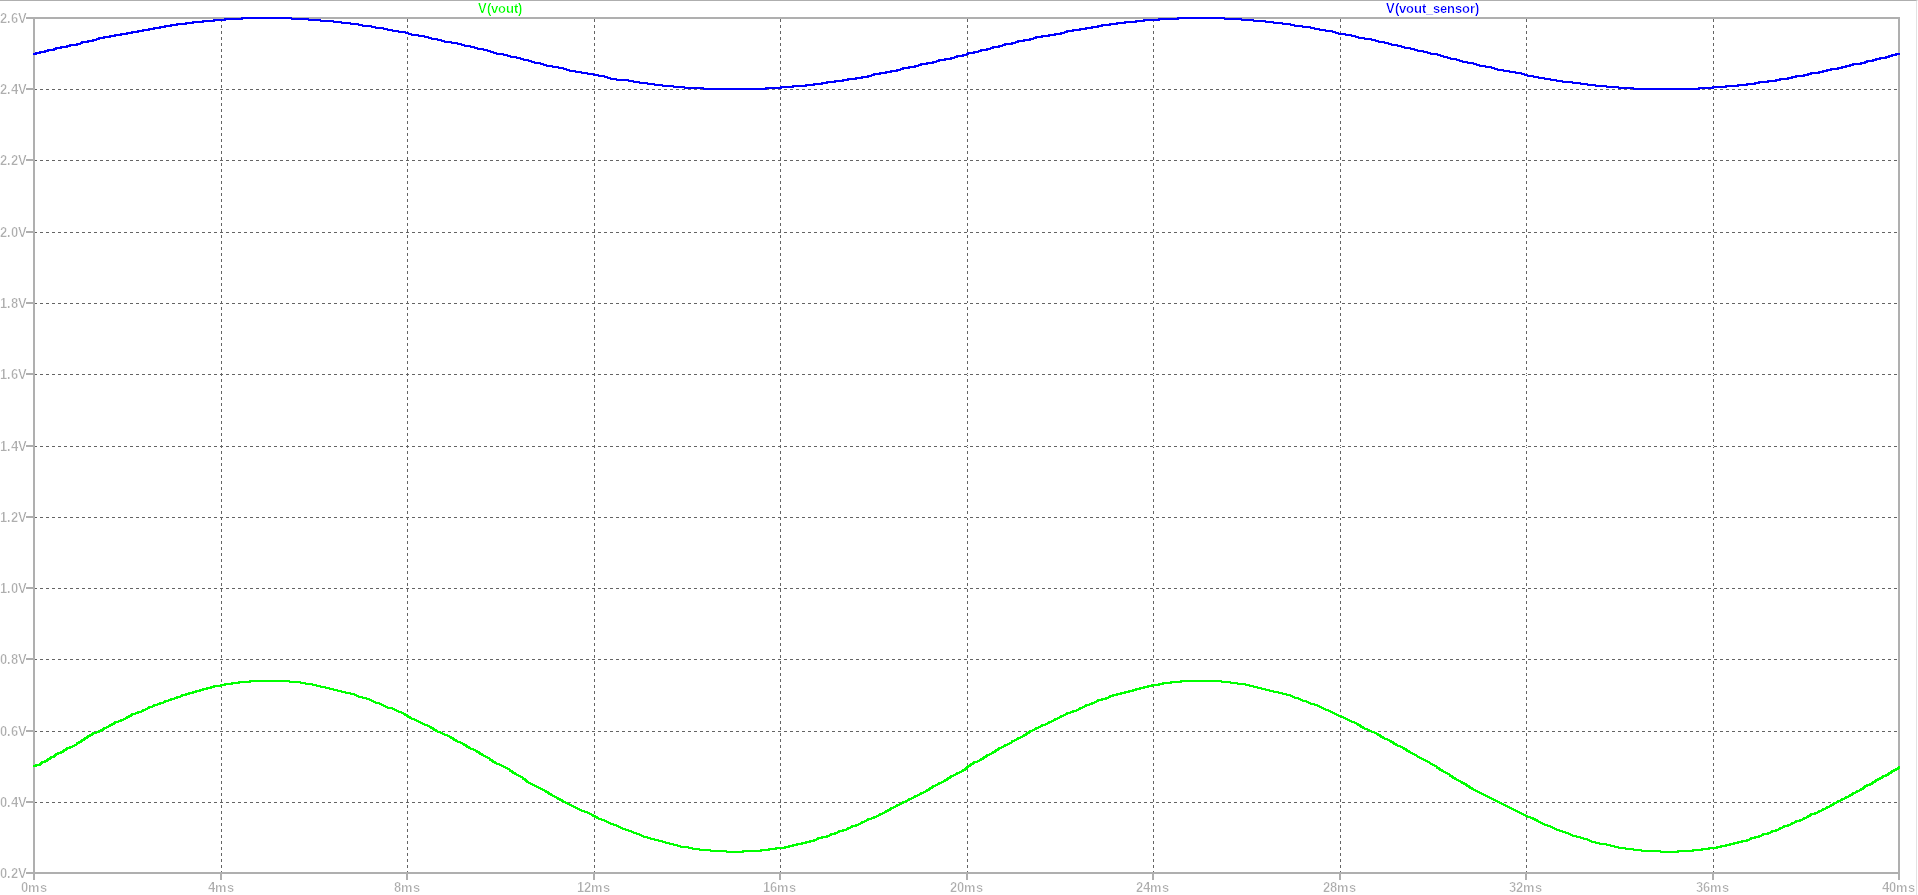
\includegraphics[width=\columnwidth]{circuito_acondicionador_sim}
	\caption{Simulación del acondicionador. La onda verde es la salida y la azul la del sensor.}
	\label{fig:acond_sim}
\end{figure}

\section{Caracterización del banco y seguridad}
\label{sec:banco}

\subsection{Equipo y valores nominales}
\label{sec:equipo}
El montaje usa una fuente de banco con límite de corriente, de la que salen $V_{dc}$ y, por un canal aparte, los \SI{15}{V} de los drivers \pendiente{marca y modelo de la fuente}. La plataforma digital es una Basys~3 con el MicroBlaze V a \SI{100}{MHz}. Las magnitudes se miden con un osciloscopio DSO-X 2002A, un multímetro 34405A y una sonda de corriente \pendiente{modelo de la sonda de corriente y de las sondas de tensión}, y las compuertas se capturan además con un analizador lógico. La Tabla~\ref{tab:nominales} reúne los valores nominales de diseño.

\begin{table}[!ht]
	\centering
	\caption{Valores nominales del montaje.}
	\label{tab:nominales}
	\begin{tabular}{lc}
		\toprule
		Magnitud & Valor nominal \\
		\midrule
		Tensión de bus $V_{dc}$ & \SI{18}{V} (\num{12} a \SI{24}{V}) \\
		Alimentación de los drivers & \SI{15}{V} \\
		Frecuencia de conmutación & \SI{20}{kHz} \\
		Período de muestreo & \SI{50}{\micro s} \\
		Tiempo muerto & \SI{1}{\micro s} \\
		Precarga del bootstrap & \SI{70}{\micro s} \\
		Resistencia total $R$ & \SI{12}{\ohm} \\
		Inductancia $L$ & \SI{30}{mH} \\
		Impedancia a \SI{50}{Hz} & \SI{15.26}{\ohm}, \ang{38.1} \\
		Fusible de entrada & \SI{630}{mA} \\
		Límite de la fuente, ensayos & \SI{0.52}{A} \\
		Umbral de falla & \SI{1.3}{A} \\
		\bottomrule
	\end{tabular}
\end{table}

\subsection{Procedimiento y seguridad}
\label{sec:seguridad}
Las pruebas energizadas las hacen los tres integrantes en el mismo lugar, una persona opera, otra toma datos y otra vigila la fuente y la carga, y esos roles se fijan antes de la primera energización \pendiente{asignar roles de la sesión}. La secuencia de puesta en marcha es la siguiente.

\begin{enumerate}
	\item Con $V_{dc}$ apagado y los \SI{15}{V} encendidos se comprueban las cuatro compuertas y el tiempo muerto (Sección~\ref{sec:plan}). Toda la cadena de compuertas funciona sin $V_{dc}$.
	\item Se sube $V_{dc}$ desde \SI{0}{V} con el límite de la fuente en \SI{0.1}{A}. Si una pierna quedó en cortocircuito, la fuente entra en limitación con pocos voltios y el electrolítico no llega a cargarse.
	\item Con el puente funcionando, se sube el límite a \SI{0.52}{A}, por debajo de la nominal del fusible, para que ante una falla sostenida limite primero la fuente.
	\item Los ensayos empiezan en \SI{12}{V} y \SI{0.2}{A}, y se sube a \SI{18}{V} y \SI{1.0}{A} solo si el paso anterior sale bien.
\end{enumerate}

La desconexión ante falla la hace el software, que baja las cuatro compuertas cuando la corriente supera \SI{1.3}{A}, cuando la cuenta del ADC cae fuera de \num{16} a \num{4079}, o cuando faltan más de tres muestras seguidas. La falla no rearma sola. Se prueba con un umbral bajo en vacío, y con una sobrecorriente real con el PR corriendo \pendiente{registrar la prueba de falla}. Una resistencia de \SI{100}{k\ohm} entre compuerta y fuente mantiene apagado cada MOSFET si el driver pierde su alimentación. El orden de apagado es bajar $V_{dc}$ y después los \SI{15}{V}.

\section{Interfaz con la plataforma digital}
\label{sec:interfaz}
El regulador se ejecuta en el MicroBlaze V y el puente lo maneja un periférico PWM propio. Para el lado de potencia, las señales que importan son pocas.

\begin{itemize}
	\item Las cuatro compuertas salen por el Pmod JA, activas en alto, todas desde flip-flops. El periférico recibe un único $d$ con signo en formato Q2.14, y la pierna B se compara contra $-d$.
	\item El valor de $d$ que se escribe a mitad de período entra a la portadora en el valle siguiente. La portadora corre aunque el puente esté apagado, y un registro de estado indica cuándo el puente conmuta de verdad.
	\item Un pulso de disparo sale en el valle de la portadora y lanza la conversión del XADC, con lo que la corriente se muestrea una vez por período de conmutación.
	\item Un temporizador interrumpe cada \num{5000} ciclos de \SI{100}{MHz}, \SI{50}{\micro s}. En cada interrupción se lee la corriente, se calcula el PR y se escribe $d$.
	\item La amplitud de la referencia sale de dos interruptores de la placa, con \num{0.2}, \num{0.5} y \SI{1.0}{A} pico, y un botón habilita el control. Otro botón exporta por UART el histórico de \num{2048} muestras, que cubre \num{5.12} períodos de \SI{50}{Hz}.
\end{itemize}

El control solo se habilita con la frecuencia de \SI{20}{kHz}. Las de \num{10} y \SI{40}{kHz} existen para mostrar el PWM sin cerrar el lazo, y el cuarto código de \texttt{freq\_sel} (11) queda igual que \SI{20}{kHz}, como se midió en las compuertas.

\section{Modelo de la planta}
\label{sec:modelo}

\subsection{Tensión promedio y función de transferencia}
\label{sec:ft}
La ley de tensiones sobre la carga da $v_o=Ri+L\,di/dt$. Con $\bar v_o=V_{dc}d$, la planta que ve el controlador es
\begin{equation}
	\frac{I(s)}{D(s)}=\frac{V_{dc}}{Ls+R},
	\label{eq:planta}
\end{equation}
con un polo en $R/L=\SI{400}{rad/s}$, un corte de \SI{64}{Hz}. La constante de tiempo, $\tau=L/R=\SI{2.5}{ms}$, es cincuenta veces el período de conmutación, y por eso el modelo promedio es válido y el rizado se calcula aparte. El núcleo del PWM carga $d$ en el valle de la portadora y lo mantiene un período, y la corriente entre muestras es una exponencial. La planta discreta con retenedor de orden cero es
\begin{equation}
	i[k+1]=a\,i[k]+b\,d[k],\quad a=e^{-T_s/\tau},\quad b=\tfrac{V_{dc}}{R}(1-a).
	\label{eq:discreta}
\end{equation}
El valor de $d$ que se calcula en la muestra $k$ entra al PWM en el valle siguiente, así que el lazo lleva un período de cómputo más medio de actualización, un retardo $T_d=1.5\,T_s=\SI{75}{\micro s}$. Es el modelo habitual de los lazos digitales de corriente y se mantiene como supuesto hasta medir el retardo real (informe técnico).

\subsection{Rizado de conmutación}
\label{sec:rizado}
Durante un pulso de $+V_{dc}$ la bobina ve $V_{dc}(1-d)$, y el pulso dura $d/(2f_{sw})$, de donde
\begin{equation}
	\Delta i_{pp}=\frac{V_{dc}\,d(1-d)}{2Lf_{sw}},\qquad
	\Delta i_{max}=\frac{V_{dc}}{8Lf_{sw}}.
	\label{eq:rizado}
\end{equation}
La fórmula es una derivación propia, y la duplicación efectiva de la frecuencia es la que traen los libros \cite{mohan2003power,hart2011}. Con \SI{18}{V}, \SI{20}{kHz} y \SI{30}{mH}, $\Delta i_{max}=\SI{3.75}{mA}$. Con \SI{24}{V} sube a \SI{5}{mA}, y a \SI{10}{kHz} se duplica. Ninguno de los tres se acerca al límite de \SI{0.20}{A}.

\subsection{Elección de la frecuencia de conmutación}
\label{sec:fsw}
La frecuencia queda entre un piso que pone el rizado y un techo que ponen el tiempo muerto y el bootstrap. El piso sale de $f_{sw}\ge V_{dc}/(8L\cdot\SI{0.20}{A})$ y con la carga vigente es de unos \SI{0.4}{kHz}, irrelevante. El techo importa más. La pérdida por tiempo muerto, $\Delta d=2T_Mf_{sw}$, es \num{0.04} a \SI{20}{kHz} y \num{0.08} a \SI{40}{kHz}, y el índice máximo del regulador baja de \num{0.92} a \num{0.84}. A \SI{40}{kHz} el escalón de \num{0.2} a \SI{1.0}{A} y el cambio de $R$ saturan el regulador, y a \SI{20}{kHz} no. A \SI{10}{kHz} el retardo extra de \SI{75}{\micro s} lleva el margen de ganancia por debajo de \SI{6}{dB}. Se eligió \SI{20}{kHz}.

\subsection{Efecto del tiempo muerto y de $R_{DS(on)}$}
\label{sec:tm_modelo}
Durante el tiempo muerto la corriente de la bobina circula por un diodo de cuerpo, y el valor de la pierna lo fija el signo de la corriente y no el PWM. La tensión promedio pierde $\Delta v=2V_{dc}T_Mf_{sw}=\SI{0.72}{V}$ en el sentido de la corriente, una onda cuadrada en fase con ella cuya fundamental vale $4\Delta v/\pi=\SI{0.92}{V}$ \cite{mohan2003power}. Además, en cualquier estado conducen dos MOSFET en serie con la carga, que suman hasta \SI{0.4}{\ohm} a $R$. Con ambos efectos, la corriente en lazo abierto resulta menor que la pedida (Tabla~\ref{tab:lazo_abierto}). La pérdida es casi una tensión fija, y pesa más cuanto menos tensión pide la referencia.

\begin{table}[!ht]
	\centering
	\caption{Predicción del ensayo en lazo abierto con \SI{18}{V}, tiempo muerto de \SI{1}{\micro s} y $R_{DS(on)}$ total de \SI{0.4}{\ohm}.}
	\label{tab:lazo_abierto}
	\begin{tabular}{cccc}
		\toprule
		Pedida (A) & Predicha (A) & Diferencia (\%) & Desfase (°) \\
		\midrule
		\num{0.2} & \num{0.146} & $-27$ & $-26.8$ \\
		\num{0.5} & \num{0.442} & $-12$ & $-33.1$ \\
		\num{1.0} & \num{0.932} & $-7$ & $-35.2$ \\
		\bottomrule
	\end{tabular}
\end{table}

Los valores salen de resolver $I=(V_{dc}m-0.92\,e^{j\varphi_I})/Z'$ en \SI{50}{Hz}, con $\varphi_I$ el ángulo de la propia corriente y $Z'$ la impedancia con los \SI{0.4}{\ohm}, por iteración de punto fijo. El modelo supone que el error cambia de signo justo cuando la corriente cruza por cero. Cerca del cruce eso no ocurre, porque mientras $|V_{dc}d|<\SI{0.72}{V}$ el tiempo muerto se lleva toda la tensión aplicada y la corriente queda en cero. En ese tramo el error copia a la tensión de referencia, así que la pérdida real es algo menor y su fundamental queda más en fase con la tensión.

\subsection{Modelo conmutado en PLECS}
\label{sec:plecs}
El modelo conmutado reproduce el puente, la modulación del núcleo del PWM, el tiempo muerto y la carga. Cada transistor es un interruptor ideal con resistencia de conducción y su diodo en antiparalelo. La portadora va de $-1$ a $1$, y el tiempo muerto se arma con dos portadoras iguales corridas $\pm2f_{sw}T_M$, una para las compuertas altas y otra para las bajas. Todos los parámetros salen de un solo archivo de Octave. La fundamental y el desfase se calculan proyectando sobre un seno y un coseno de \SI{50}{Hz} en cuatro períodos completos, y el rizado se mide restando a la corriente su promedio por período de conmutación.

El modelo se validó con la carga anterior de \SI{10}{\ohm} y \SI{2}{mH}, con $V_{dc}=\SI{18}{V}$ y una referencia de \SI{0.2}{A} (Tabla~\ref{tab:plecs}). Sin tiempo muerto ni $R_{DS(on)}$ el modelo entrega la corriente que fija la impedancia de la carga, así que el puente y el modulador no agregan error. Con tiempo muerto la amplitud queda a \SI{2}{\percent} del análisis y el desfase no, por el tramo de corriente nula descrito arriba. El modelo no se volvió a correr con la carga vigente, y esa validación está \pendiente{repetir la validación en PLECS con 12 $\Omega$ y 30 mH}.

\begin{table}[!ht]
	\centering
	\caption{Modelo en PLECS contra el análisis, con la carga anterior (\SI{10}{\ohm}, \SI{2}{mH}) y \SI{0.2}{A}.}
	\label{tab:plecs}
	\begin{tabular}{lcccc}
		\toprule
		Caso & $I$ PLECS (A) & $\varphi$ (°) & $I$ análisis (A) & $\varphi$ (°) \\
		\midrule
		Sin $T_M$ ni $R_{DS}$ & \num{0.2000} & \num{3.60} & \num{0.2000} & \num{3.60} \\
		Solo $R_{DS(on)}$ & \num{0.1923} & \num{3.46} & \num{0.1923} & \num{3.46} \\
		Solo $T_M$ & \num{0.1104} & \num{3.48} & \num{0.1086} & \num{1.95} \\
		Los dos & \num{0.1062} & \num{3.35} & \num{0.1044} & \num{1.88} \\
		\bottomrule
	\end{tabular}
\end{table}

\section{Diseño del regulador PR}
\label{sec:pr}

\subsection{Estructura y sintonización}
\label{sec:estructura}
Se usa la estructura ideal $G_c(s)=K_p+K_r\,s/(s^2+\omega_0^2)$ con $\omega_0=2\pi\cdot\SI{50}{Hz}$. La versión amortiguada cambia exactitud en \SI{50}{Hz} por tolerancia a que la frecuencia se corra, y aquí la referencia la genera el propio procesador a \SI{50}{Hz} exactos, así que la ideal no pierde nada \cite{teodorescu2006}.

El lazo abierto es $L(s)=G_c(s)\,e^{-sT_d}/(Ls+R)$. Se fija el ancho de banda en $f_c=f_s/20=\SI{1}{kHz}$. Con más ancho de banda el retardo de $T_d$ come margen, y con menos la parte proporcional se vuelve lenta. Como el resonante aporta poco en el cruce ($K_r/\omega_c\approx0.48$), $K_p$ se calcula como si no estuviera, imponiendo ganancia unitaria en $\omega_c$,
\begin{equation}
	K_p=\sqrt{R^2+(\omega_cL)^2}=\SI{188.88}{V/A}.
	\label{eq:kp}
\end{equation}
Con la carga anterior $K_p$ era de \SI{16.06}{V/A}. Con \SI{30}{mH}, $\omega_cL=\SI{188.5}{\ohm}$ domina sobre $R$, y por eso $K_p$ subió casi doce veces. Es la causa de la saturación que se discute en la Sección~\ref{sec:sat}, y no un ajuste cosmético.

$K_r$ fija qué tan rápido converge el error en \SI{50}{Hz}. Se simuló un lazo discreto completo (planta por retenedor de orden cero, un muestreo de retardo, regulador con Tustin precorregido) con un escalón de \num{0.2} a \SI{1.0}{A} aplicado en un cruce por cero. El error de amplitud de la fundamental por período es de \num{5.8}, \num{5.5}, \num{5.2}, \num{4.9} y \SI{4.7}{\percent} con $K_r=1000$, de \num{5.3}, \num{4.6}, \num{3.9}, \num{3.4} y \SI{2.9}{\percent} con $K_r=3000$, y de \num{5.0}, \num{3.9}, \num{3.0}, \num{2.3} y \SI{1.8}{\percent} con $K_r=5000$. Se eligió $K_r=3000$. Con esta carga hasta \num{1000} alcanza, y se conservó \num{3000} porque era el valor de la carga anterior y deja margen si el $K_p$ real resulta menor, a un costo casi nulo en margen de fase.

\subsection{Discretización}
\label{sec:disc}
El resonante discretizado es un filtro de segundo orden, $r[k]=b_0e[k]+b_1e[k-1]+b_2e[k-2]-a_1r[k-1]-a_2r[k-2]$. Con Tustin simple el polo se corre por debajo de \SI{50}{Hz}. Se usa Tustin con precorrección en $\omega_0$, $s=\frac{\omega_0}{\tan(\omega_0T_s/2)}\frac{z-1}{z+1}$, que cuesta lo mismo, deja el polo exactamente en \SI{50}{Hz} a cualquier $f_s$ y da los coeficientes en forma cerrada \cite{yepes2010}. Con $\theta=\omega_0T_s$,
\begin{equation}
	b_0=\frac{K_r\sin\theta}{2\omega_0},\ b_1=0,\ b_2=-b_0,\ a_1=-2\cos\theta,\ a_2=1.
	\label{eq:coef}
\end{equation}
Dividiendo $K_p$ entre $V_{dc}=\SI{24}{V}$ para que la salida sea índice de modulación, los coeficientes finales son $K_P=\num{7.8699}$, $b_0=\num{3.1249e-3}$, $b_2=-\num{3.1249e-3}$ y $a_1=-\num{1.99975}$. Se divide entre \SI{24}{V}, el máximo del enunciado, porque el $1/V_{dc}$ queda fijo en el programa y el bus real lo vuelve a multiplicar. Con el bus más bajo el lazo solo pierde ganancia, y con coeficientes de \SI{18}{V} y el bus en \SI{24}{V} la esquina de $L$ baja quedaría en \ang{40.5} y \SI{5.0}{dB}. Además, con el tiempo muerto, la $R_{DS(on)}$ y la carga medida de \SI{12.5}{\ohm}, \SI{1.0}{A} con \SI{18}{V} pide un índice de \num{0.929}, sobre $\num{0.92}$, así que el lazo cerrado se ensaya con \SI{24}{V}, donde queda en \num{0.707}. $a_1$ queda muy cerca de $-2$ y la diferencia con $-2$ fija la frecuencia del polo, así que hay que representarla bien. En punto flotante de \num{32} bits el paso en ese valor es de \num{1.2e-7}, que corre el polo \SI{0.012}{Hz} y deja la ganancia del resonante en \SI{50}{Hz} en miles. Por eso el controlador corre en punto flotante en el procesador.

\subsection{Saturación y rampa de amplitud}
\label{sec:sat}
La salida del regulador se recorta a $\pm0.92$, y si hubo recorte el estado del resonante se corrige para que no acumule energía mientras el puente está saturado (anti-windup). En régimen, \SI{1.0}{A} con \SI{18}{V} pide \num{0.848} y no satura. El problema es el escalón de amplitud, que en el sistema real lo aplican los interruptores de selección, a mano y en cualquier fase de la senoidal. Con la carga vigente, el escalón de \num{0.2} a \SI{1.0}{A} en la peor fase pide un índice de hasta \num{8.53} con \SI{18}{V}, y con $12\,\mathrm{V}$ llega a \num{12.80}. Con la saturación y el anti-windup del código real, el error de la fundamental queda en \num{11.6}, \num{36.9} y \SI{58.1}{\percent} en los tres primeros períodos, y ningún $K_r$ entre \num{3000} y \num{30000} baja el segundo período de \SI{10}{\percent}. El anti-windup evita que el resonante se descontrole, pero no puede hacer que el puente entregue más tensión que su tope.

La salida fue limitar la velocidad de cambio de la amplitud de la referencia, y no tocar $K_p$ ni $K_r$. Una rampa de \num{200} muestras (medio período) no alcanza, con \SI{12.2}{\percent} de error en el segundo período en la peor de \num{20} fases del escalón, medido contra la amplitud que pide el interruptor y no contra la rampeada. Con \num{400} muestras (\SI{20}{ms}, un período completo) el peor caso baja a \SI{4.0}{\percent} en el segundo período y \SI{3.5}{\percent} en el tercero, con un pico de corriente de \SI{0.979}{A}. Entre \num{350} y \num{480} muestras el resultado es parecido, y con \num{800} o más vuelve a subir (\SI{14.9}{\percent} a \num{800}), porque la corriente pasa demasiado tiempo en amplitudes intermedias. La rampa quedó en \num{400} muestras.

\subsection{Estabilidad}
\label{sec:estab}
El diseño nominal cruza en \SI{1.0}{kHz} con \ang{66.5} de margen de fase y \SI{10.5}{dB} de margen de ganancia (Fig.~\ref{fig:bode}). Se pide al menos \ang{45} y \SI{6}{dB}, y en las esquinas de $L$ (\SI{\pm30}{\percent}) y $R$ (\SI{\pm25}{\percent}) con $K_p$ sin retocar al menos \ang{30} y \SI{3}{dB}. Las cuatro esquinas cumplen, con \ang{54.0} y \SI{7.5}{dB} en la peor ($L=\SI{21}{mH}$, $R$ de \num{9} o \SI{15}{\ohm}), porque con menos $L$ sube el cruce y la carga aporta menos fase.

\begin{figure}[!ht]
	\centering
	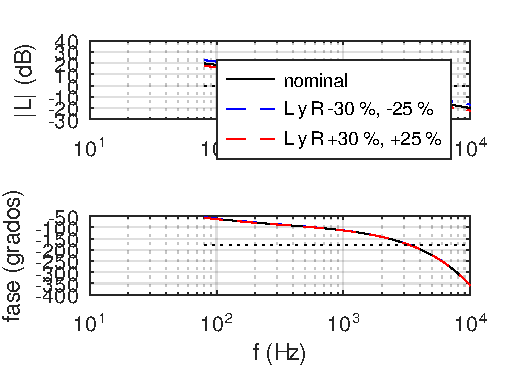
\includegraphics[width=\columnwidth]{bode_lazo}
	\caption{Lazo abierto, nominal y esquinas de $L$ y $R$, con el retardo de \SI{75}{\micro s}. Las líneas de puntos son \SI{0}{dB} y $-\ang{180}$.}
	\label{fig:bode}
\end{figure}

El retardo adicional es lo que más mueve los márgenes (Fig.~\ref{fig:retardo}). Con \SI{25}{\micro s} extra quedan \ang{57.5} y \SI{8.1}{dB}, con \SI{50}{\micro s} \ang{48.5} y \SI{6.2}{dB}. El margen de ganancia llega a \SI{6}{dB} con \SI{53}{\micro s} de más y el de fase llega a \ang{45} con \SI{60}{\micro s}, y los dos límites quedan casi juntos. Entre el aislamiento de las compuertas, de pocos microsegundos como mucho, y el filtro del sensor, ya no sobra margen para cualquier valor. Con un RC de primer orden en el sensor, el nominal da \ang{56.0} y \SI{8.6}{dB} con corte en \SI{5}{kHz}, \ang{50.3} y \SI{8.2}{dB} con \SI{3}{kHz}, y \ang{44.8} y \SI{7.9}{dB} con \SI{2}{kHz}, que ya queda bajo el mínimo de fase por una décima. En la esquina de $L=\SI{21}{mH}$ y $R=\SI{9}{\ohm}$, el RC de \SI{2}{kHz} no cumple (\ang{28.8} contra \ang{30}). El filtro propuesto de \SI{4823}{Hz} equivale al de \SI{5}{kHz}.

\begin{figure}[!ht]
	\centering
	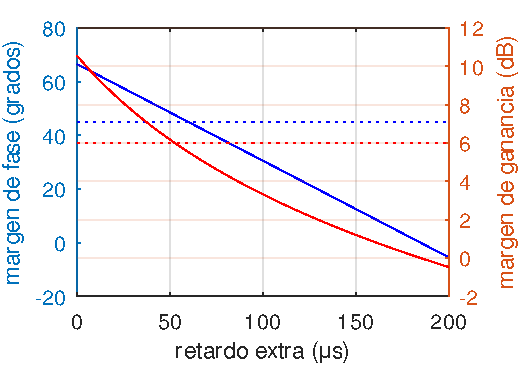
\includegraphics[width=\columnwidth]{margenes_retardo}
	\caption{Margen de fase y de ganancia contra el retardo agregado a los \SI{75}{\micro s} del modelo. Las líneas de puntos son los mínimos de \ang{45} y \SI{6}{dB}.}
	\label{fig:retardo}
\end{figure}

\subsection{Muestreo y aliasing}
\label{sec:alias}
La señal de \SI{50}{Hz} y el cruce de \SI{1}{kHz} quedan muy por debajo de $f_s/2$. Lo que el criterio $f_s>2BW$ no mira es el resto de lo que entra al ADC. Si la conversión cae en el valle o en el pico de la portadora, el rizado de conmutación es un múltiplo exacto de $f_s$ en ese instante y se pliega a continua, con poco efecto en la amplitud. Por eso el núcleo del PWM emite un pulso de disparo en el valle, y el XADC convierte cuando lo recibe. Se simuló el puente conmutado con la carga vigente, la portadora de \num{2500} cuentas y el PR de las secciones anteriores. El error de amplitud de la fundamental de la corriente verdadera, no la muestreada, no pasa de \SI{0.20}{\percent} en ningún instante de captura probado. Con la captura en el valle da \SI{-0.09}{\percent}, igual con \num{1.0} y \SI{0.2}{A}, y con \SI{0.91}{\micro s} de adelanto, el máximo retardo de la cadena de compuertas, \SI{-0.13}{\percent}. En el flanco del pulso da \SI{-0.01}{\percent}, y con una fase cualquiera a \num{5}, \num{7.8} y \SI{20}{\micro s} del valle, \num{0.02}, \SI{-0.01}{\percent} y \SI{-0.20}{\percent}. Con la bobina de \SI{2}{mH} esos mismos puntos llegaban a \SI{2.8}{\percent}, y el cambio se debe a que el rizado es quince veces menor. El corrimiento común de unos \SI{-0.09}{\percent} no depende del instante y viene de la discretización del lazo.

El ruido de banda ancha del sensor y de la conmutación no se sincroniza con nada, y solo lo frena un filtro analógico, que a su vez agrega un retardo $\tau_F=1/(2\pi f_F)$ al lazo (Sección~\ref{sec:estab}).

\section{Simulación del lazo}
\label{sec:sim}
Se simuló el lazo discreto promedio con $L=\SI{30}{mH}$, $R=\SI{12}{\ohm}$, $K_p=\SI{188.88}{V/A}$ y $K_r=3000$, y se midió el error de amplitud de la fundamental, $(|I_1|-|R_1|)/|R_1|$ en valor absoluto, con ventanas de un período y los fasores extraídos proyectando sobre seno y coseno. Es el criterio del enunciado. Estos resultados valen para un escalón aplicado en el cruce por cero y no incluyen rizado de conmutación, cuantización del ADC, ruido del sensor ni tiempo muerto. Salen de \texttt{verificar\_pr.m}, y las figuras de \texttt{figuras\_informe.m}.

\begin{table}[!ht]
	\centering
	\caption{Error de amplitud de la fundamental por período tras el cambio, en porcentaje, con $K_r=3000$.}
	\label{tab:err_sim}
	\begin{tabular}{lccccc}
		\toprule
		Cambio & 1 & 2 & 3 & 4 & 5 \\
		\midrule
		\num{0.2} a \SI{0.5}{A} & \num{5.2} & \num{4.5} & \num{3.8} & \num{3.3} & \num{2.8} \\
		\num{0.5} a \SI{1.0}{A} & \num{5.1} & \num{4.4} & \num{3.8} & \num{3.2} & \num{2.8} \\
		\num{0.2} a \SI{1.0}{A} & \num{5.3} & \num{4.6} & \num{3.9} & \num{3.4} & \num{2.9} \\
		$R$ de \num{12} a \SI{15}{\ohm}, \SI{0.5}{A} & \num{1.4} & \num{1.2} & \num{1.0} & \num{0.9} & \num{0.8} \\
		\bottomrule
	\end{tabular}
\end{table}

El cambio de $R$ de \SI{25}{\percent} se aplica con el lazo ya en régimen, y el error es más chico que con los escalones porque $K_p$ domina el seguimiento. En las esquinas de $L$ y $R$ el peor error es \SI{6.6}{\percent} en el primer período y \SI{4.9}{\percent} en el segundo. Solo con la parte proporcional, el error de amplitud es de \SI{6.0}{\percent}, con un desfase de \ang{-2.8}. Con el tiempo muerto y la $R_{DS(on)}$ se espera, solo con proporcional, un error de \num{8.4}, \num{7.1} y \SI{6.6}{\percent} con \num{0.2}, \num{0.5} y \SI{1.0}{A}, y un desfase de \ang{-2.7} a \ang{-2.8}.

\begin{figure}[!ht]
	\centering
	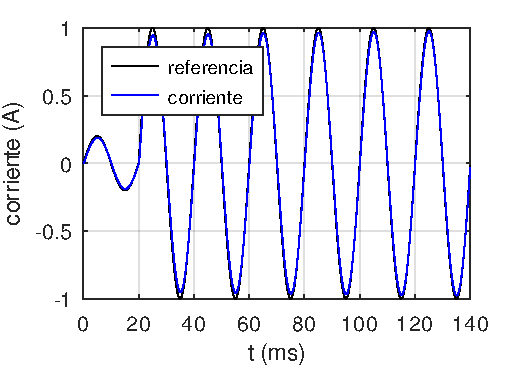
\includegraphics[width=\columnwidth]{escalon_02_10}
	\caption{Escalón de \num{0.2} a \SI{1.0}{A} aplicado en un cruce por cero, en el lazo promedio sin saturación. El primer período es el arranque desde cero.}
	\label{fig:escalon}
\end{figure}

\begin{figure}[!ht]
	\centering
	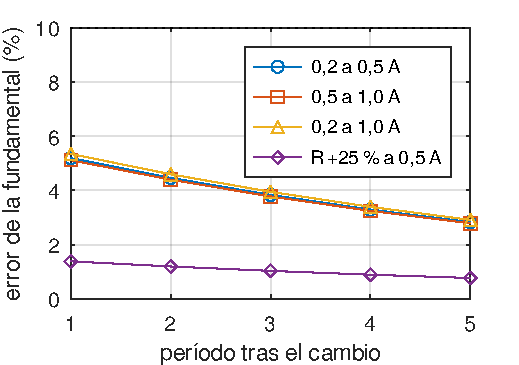
\includegraphics[width=\columnwidth]{error_escalones}
	\caption{Error de la fundamental por período tras cada cambio. La línea de puntos es el límite de \SI{10}{\percent}.}
	\label{fig:err}
\end{figure}

\section{Plan de validación y procedimiento de medición}
\label{sec:plan}
Cada paso descarta una causa antes de sumar la siguiente. Primero se prueba sin energizar y después se sube la potencia por pasos. Los ensayos con la potencia aplicada los hacen tres personas en el mismo lugar, una opera y otra toma datos, y se arranca con $V_{dc}=\SI{12}{V}$ y \SI{0.2}{A}. Con \SI{1.0}{A} no se baja de \SI{18}{V}.

\subsection{Antes de energizar}
Se verifican las cuatro compuertas y el tiempo muerto con la potencia apagada, con osciloscopio y con analizador lógico. Esta prueba se hizo el 16 de noviembre con el osciloscopio, y su resultado está en el informe técnico. Los criterios son el período de \SI{50}{\micro s} en cada pierna, el tiempo muerto de \SI{1}{\micro s} en los dos flancos de las dos piernas, ninguna conducción simultánea de alta y baja de una misma pierna en una captura larga, incluso al arrancar y al apagar, y los pulsos de las dos piernas centrados en el valle de la portadora. Con \SI{0}{A} en la carga, el ADC debe dar la cuenta de offset (\num{2048}), y la corriente que mide se compara con la de una sonda. Se fija el umbral de falla y se comprueba que baje las compuertas, encienda el indicador y no rearme solo.

\subsection{Pasos energizados}
\begin{enumerate}
	\item Lazo abierto, con un $d$ senoidal fijo de \SI{50}{Hz} y sin PR. Se compara la amplitud y el desfase de la corriente con la Tabla~\ref{tab:lazo_abierto}. Si se aleja más de \SI{10}{\percent} se detiene la prueba. Sirve para validar la ganancia del sensor, el signo y los valores de $L$ y $R$. Si el tiempo muerto medido no es de \SI{1}{\micro s}, se recalcula la predicción antes de comparar.
	\item Solo la parte proporcional, con $K_r=0$.
	\item PR completo con \num{0.2}, \num{0.5} y \SI{1.0}{A} pico.
	\item Cambios de amplitud de \num{0.2} a \num{0.5} y de \num{0.5} a \SI{1.0}{A}.
	\item Cambio de $R$ de al menos \SI{25}{\percent} con \SI{0.5}{A} pico, sin disparar el umbral de falla.
\end{enumerate}

\subsection{Mediciones del lazo y evidencia}
Un pin de depuración sube al entrar a la rutina periódica y baja al salir. Con él se miden el período, que debe ser de \SI{50}{\micro s}, el jitter, la duración de la rutina y su fase contra el disparo del ADC en varios reinicios. El retardo efectivo del lazo, desde la captura hasta el cambio en las compuertas, se compara con los \SI{75}{\micro s} del modelo más $\tau_F$. De cada ensayo se guardan la referencia, la corriente, la tensión sobre la carga y las señales PWM en la misma captura, con $V_{dc}$, $R$, $L$, tiempo muerto y frecuencia, y la corrección o el fallo que hubo.

\section{Montaje y adquisición}
\label{sec:montaje}
Cada ensayo se registra por dos caminos al mismo tiempo. El osciloscopio captura la corriente de la carga, la tensión sobre la carga y las compuertas, con una ventana local de unos pocos períodos de conmutación para el rizado y otra de al menos cinco períodos de \SI{50}{Hz} para la fundamental \pendiente{muestreo y ventana de cada captura}. La corriente se mide con una sonda o un resistor de bajo valor \pendiente{método de medición de la corriente y su escala}. El histórico del controlador se toma por la UART a \num{115200} baudios, una trama de \num{12310} bytes que tarda \SI{1.07}{s}, con un registro por período de portadora, es decir a \SI{20}{kS/s}. Las compuertas y el pin de depuración de la rutina periódica se miran con un analizador lógico de \SI{24}{MHz} o más, que resuelve el tiempo muerto con unos $\pm\SI{40}{ns}$, y con el osciloscopio para el valor final.

Las dos fuentes de datos miden la corriente por caminos distintos, el sensor y el acondicionador de la placa por un lado y la sonda por el otro, y por eso se comparan. Una diferencia sistemática entre ambas apunta a la ganancia del sensor o al offset, y se corrige antes de aceptar un error de la fundamental. Los archivos de cada captura se nombran por ensayo y punto de operación, con una tabla de ventana, muestreo y escala \pendiente{tabla de archivos de captura}.

\subsection{Procesamiento}
\label{sec:proc}
La corriente se muestrea una vez por período de portadora, en el valle, así que el histórico de la ejecución no contiene el rizado de conmutación. El histórico se exporta por la UART de la placa a la PC, sin afectar el lazo. Ahí se ajusta por mínimos cuadrados una senoidal de \SI{50}{Hz} más un término constante sobre períodos enteros, y se obtienen la amplitud y el desfase de la fundamental de la corriente y de la referencia. El error de amplitud es $(|I_1|-|R_1|)/|R_1|$ sobre al menos cinco períodos. Ese error se calcula con los registros del controlador, que ven la corriente a través del sensor, y se contrasta con el osciloscopio. El rizado se mide aparte, con el osciloscopio, en una ventana local de unos pocos períodos de conmutación, restando a la corriente su promedio por período, el mismo procedimiento que se usó en el modelo conmutado. Las dos cantidades se informan por separado, y se distinguen valores pico y RMS en cada figura.

\section{Conclusiones}
\label{sec:conclusiones}
Tres decisiones pesaron más que el resto. La frecuencia de \SI{20}{kHz} deja el índice máximo en \num{0.92} y el retardo del lazo dentro del margen. El tiempo muerto de \SI{1}{\micro s} sale del peor caso de la cadena de compuertas (\SI{813}{ns}) y cuesta entre \num{7} y \SI{27}{\percent} de la corriente en lazo abierto. La rampa de un período en la referencia evita la saturación del escalón, que ni el anti-windup ni un $K_r$ mayor resuelven.

\appendix
\section{Archivos para reproducir los resultados}
\label{app:archivos}
Todas las rutas son relativas a la raíz del repositorio.

\begin{itemize}
	\item \texttt{potencia/diseno\_pr.md}, \texttt{potencia/diseno\_puente\_h.md} y \texttt{potencia/docs/modelo\_planta.md}, con el diseño del regulador, del puente y de la planta.
	\item \texttt{potencia/verificar\_pr.m} y \texttt{potencia/aliasing\_pr.m}, los cálculos y simulaciones del lazo en Octave.
	\item \texttt{potencia/informe/figuras\_informe.m}, que genera las figuras de este informe.
	\item \texttt{sw/generar\_pr\_params.m}, que escribe los coeficientes en \texttt{sw/pr\_params.h}.
	\item \texttt{potencia/sim/}, el modelo conmutado en PLECS y su archivo de parámetros.
	\item \texttt{sw/receptor\_pc.py}, el procesamiento de los registros exportados.
\end{itemize}

\printbibliography

\begin{IEEEbiography}[{
\includegraphics[width=1in,height=1.25in,clip,keepaspectratio]{jch_BN}}]{Jefferson Chinchilla-Quesada}
	Estudiante de Ingeniería Electrónica, Instituto Tecnológico de Costa Rica.
	Correo, jechinchilla@estudiantec.cr
\end{IEEEbiography}

\begin{IEEEbiography}[{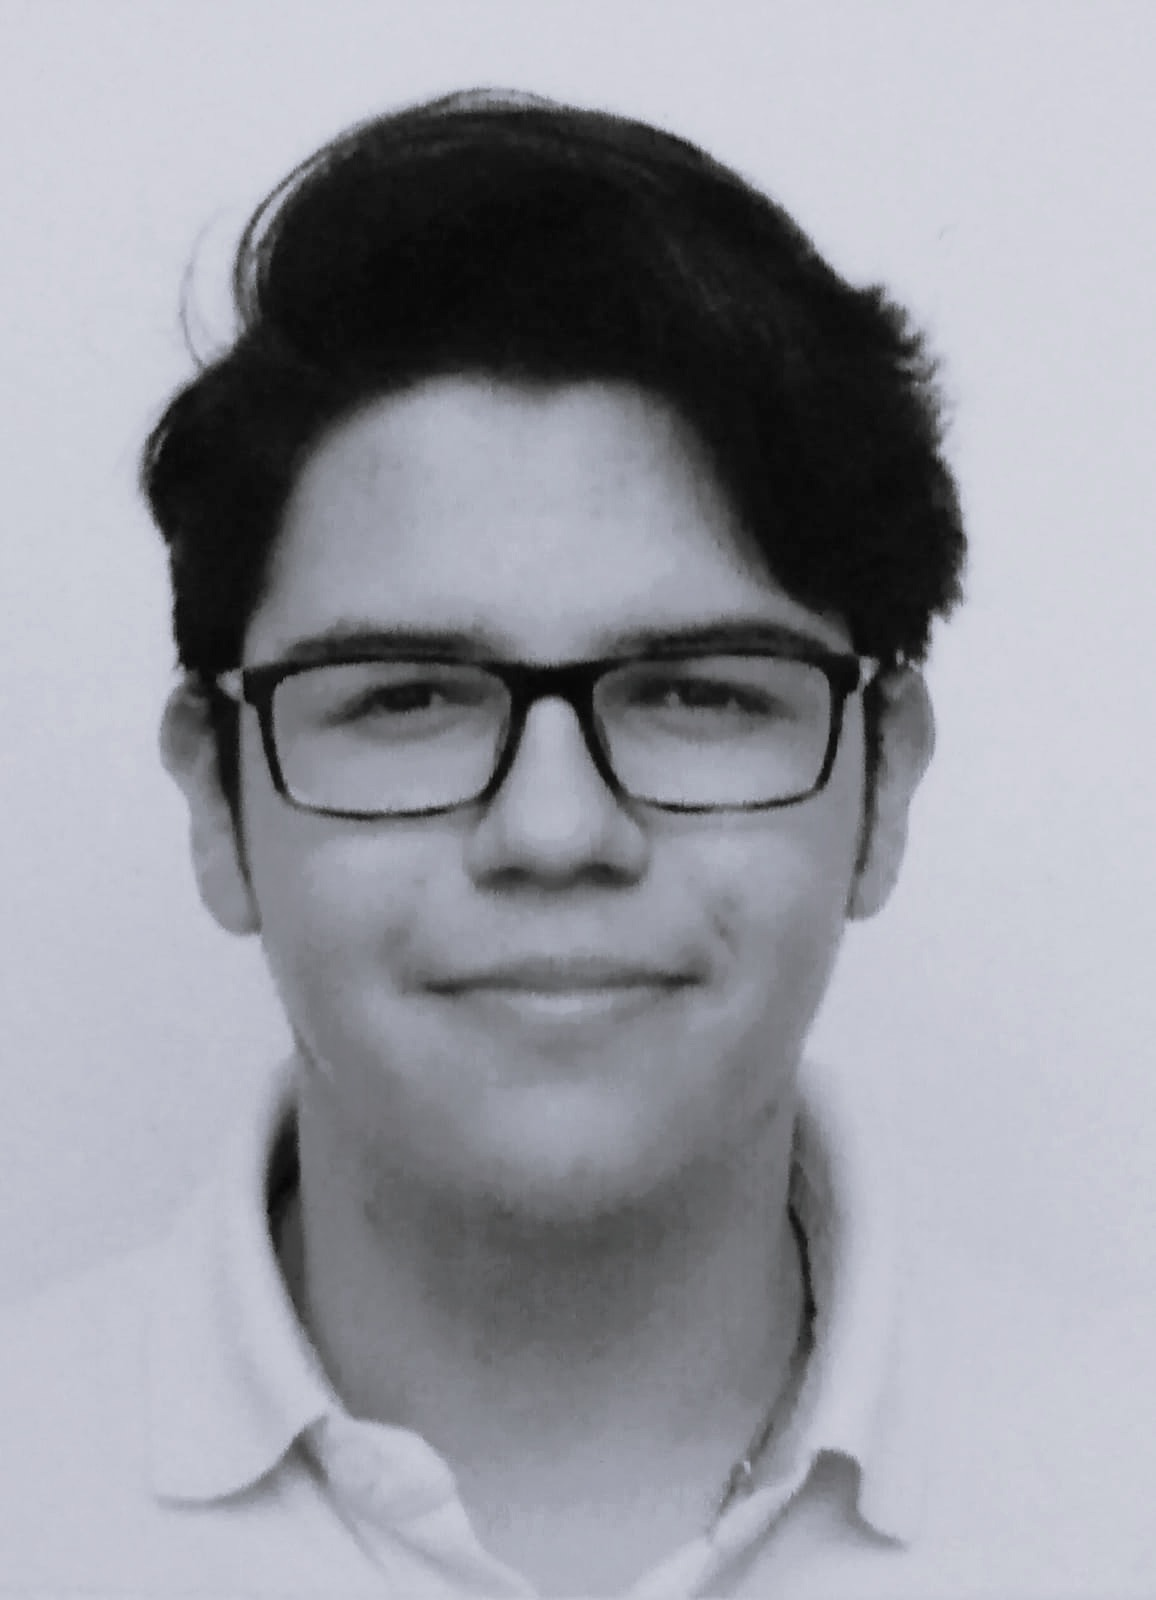
\includegraphics[width=1in,height=1.25in,clip,keepaspectratio]{nmv_bn}}]{Nicolás Mena-Valerio}
	Estudiante de Ingeniería Electrónica, Instituto Tecnológico de Costa Rica, desde 2022.
	Correo, nimena@estudiantec.cr
\end{IEEEbiography}

\begin{IEEEbiography}[{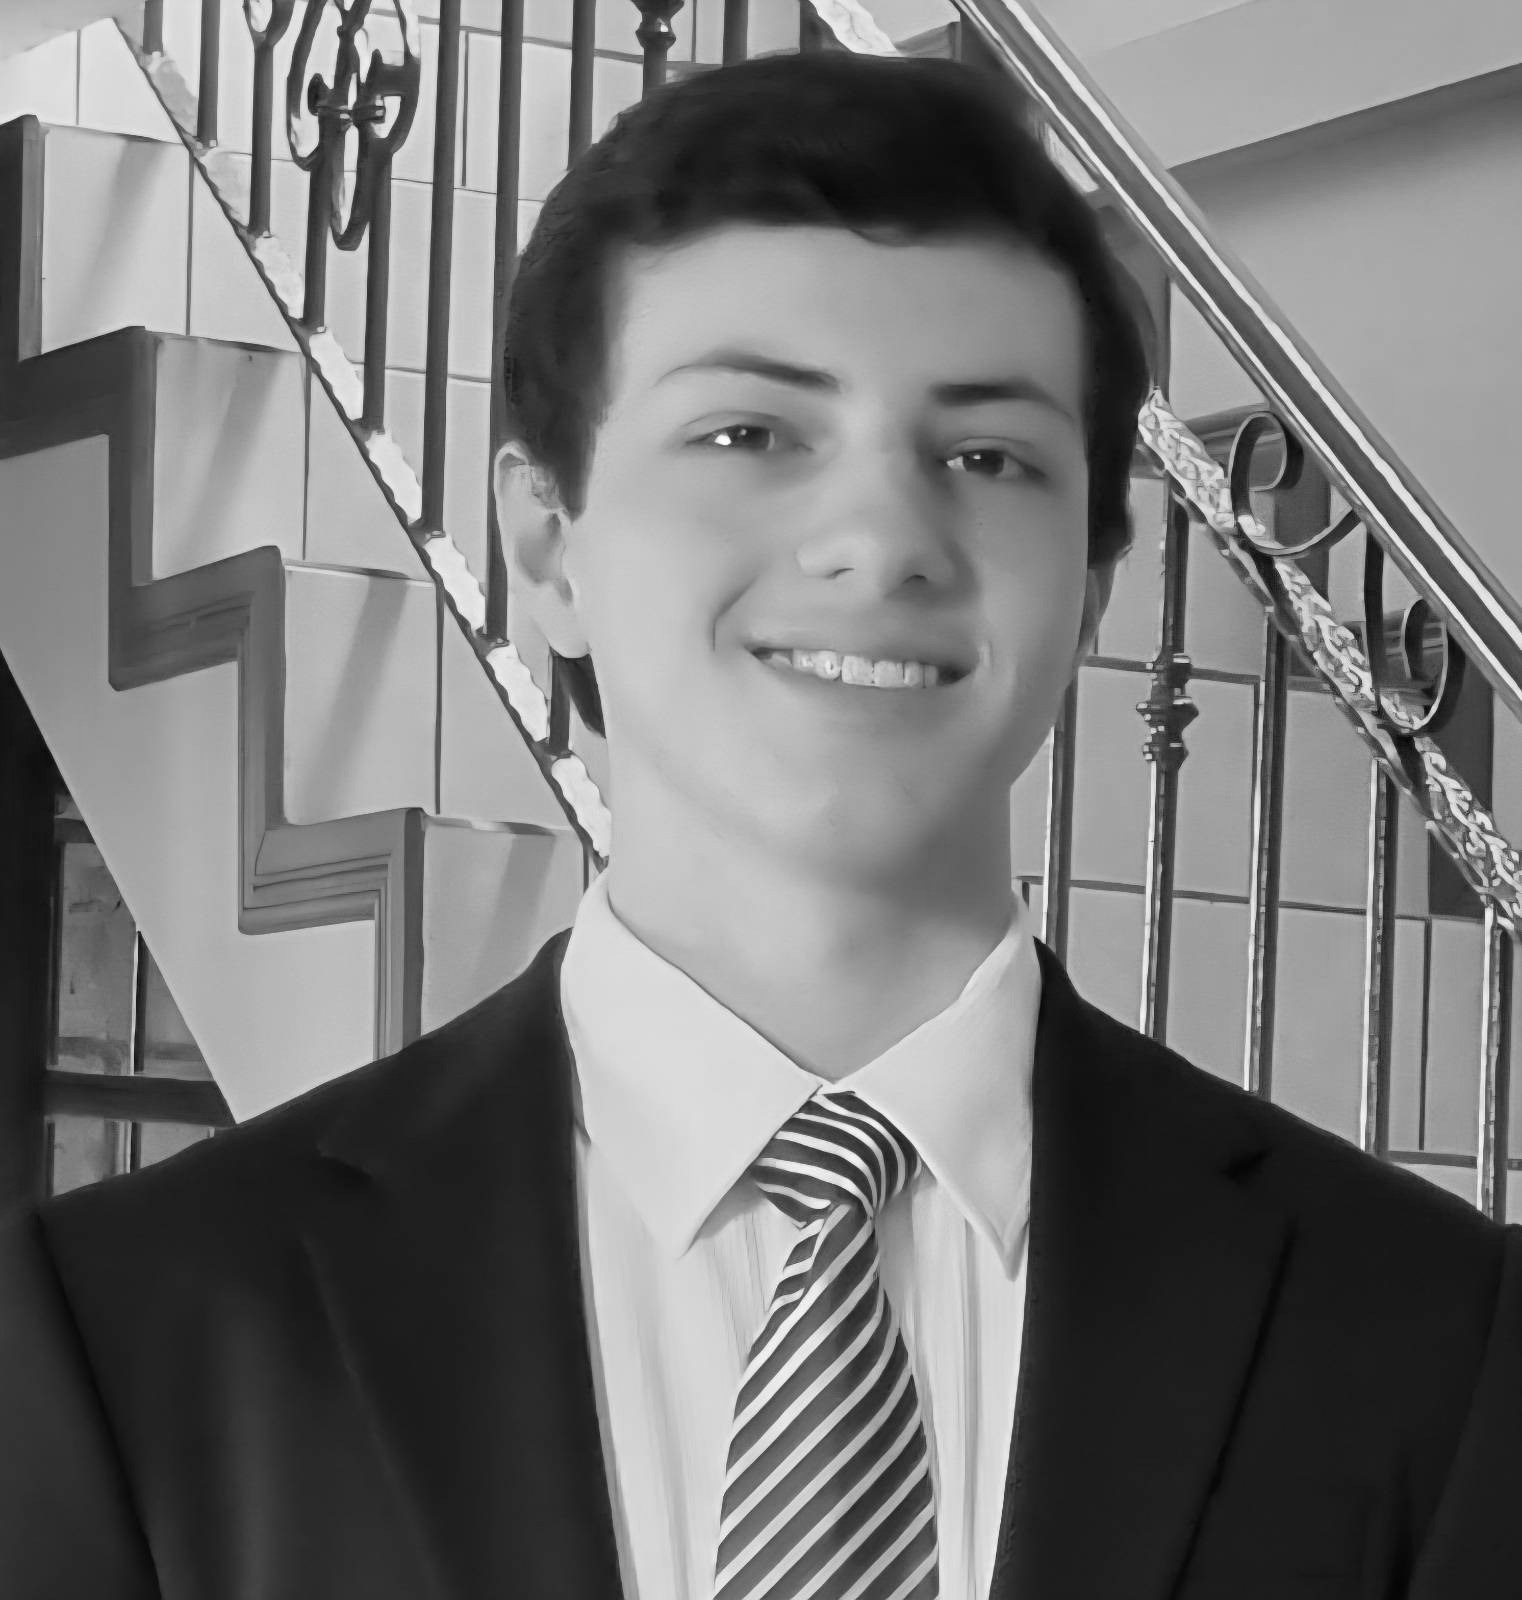
\includegraphics[width=1in,height=1.25in,clip,keepaspectratio]{mcq_bn}}]{Mattio Coghi-Quirós}
	Estudiante de Ingeniería Electrónica, Instituto Tecnológico de Costa Rica.
	Correo, mcoghi@estudiantec.cr
\end{IEEEbiography}

\vfill
\end{document}